% \vspace{-10pt}
We implemented our framework in LLVM (forked from commit $360853$ on May 15 2019).
In LLVM the OpenMP constructs are lowered to runtime calls in Clang, so 
in the LLVM IR we only see calls to the OpenMP runtime. 
There are several limitations of this approach with respect 
to high level analysis like the one OMPSan is trying to accomplish.
%disadvantages of this approach especially with respect to our analysis. 
For example, the region of code that needs to be offloaded to a device 
is opaque since it is moved to a separate function. 
These functions are in turn called from the OpenMP runtime library. 
As a result, it is challenging to perform a global data flow analysis 
for the memory def-use information of the offloaded region. 
To simplify the analysis, we have to compile with clang twice. 

First, we compile the OpenMP program with the flag that enables
parsing the OpenMP constructs, and compile it again without the flag, 
so that Clang ignores the OpenMP constructs and instead generates the 
baseline LLVM IR for the sequential version. 
During the OpenMP compilation pass, we execute 
our analysis pass, which parses the runtime library calls 
and generates a csv file that records all the user specified 
``target map'' clauses, as explained in \autoref{interpreting-openmp-pragmas}.

Next we compile the program by ignoring the OpenMP pragmas, 
and perform  whole program context and flow sensitive data flow analysis
on LLVM code generated from the sequential version, to construct
the Memory def-use chains, explained in 
\autoref{baseline-mem-def-analysis}.
Then this pass validates if the ``target map''
information recorded in the csv file, respects all the Memory 
def-use relations present in the sequential version of the code.
% \vspace{-10pt}
\subsection{Interpreting OpenMP pragmas}
\label{interpreting-openmp-pragmas}
% \vspace{-10pt}
% The offload mechanism used by clang is to generate calls to a runtime library(RTL) whenever ``target'' directives are encountered. 
% The offload library implements the routines shown in \autoref{RTL-routines}. In the LLVM IR, whenever 
% we encounter a call to one of these RTL routines, we parse the arguments of the functions, and 
% extract the relevant information from them.
% % \autoref{RTL-arguments} lists the arguments that are 
% % relevant to interpret the semantics of the \textit{map} clause.
% \begin{table}
%     \caption{Target Runtime Library Routines}
%     \label{RTL-routines}
%     \scriptsize
%     \begin{center}
%         \begin{tabular}{ |m{2in} | m{3in} |}
%             \hline
%             RTL Routines & Arguments \\ \hline    
%             
%             $\_\_tgt\_target\_data\_begin$ :: Initiate a device data environment & 
%             \begin{minipage}{3in}
%                 \begin{verbatim}
%                     
%   int64_t device_id, int32_t num_args
%   void** args_base, void** args, 
%   int64_t *args_size, int64_t *args_maptype         
%                 \end{verbatim}
%             \end{minipage}
%             \\ \hline   
%             $\_\_tgt\_target\_data\_end$ :: Close a device data environment & 
%             \begin{minipage}{3in}
%                 \begin{verbatim}
%                     
%   int64_t device_id, int32_t num_args
%   void** args_base, void** args, 
%   int64_t *args_size, int64_t *args_maptype         
%                 \end{verbatim}
%             \end{minipage}
%             \\ \hline
%             $\_\_tgt\_target\_data\_update$ :: Make a set of values consistent between host and device& 
%             \begin{minipage}{3in}
%                 \begin{verbatim}
%                     
%   int64_t device_id, int32_t num_args
%   void** args_base, void** args, 
%   int64_t *args_size, int64_t *args_maptype         
%                 \end{verbatim}
%             \end{minipage}
%             \\ \hline
%             $\_\_tgt\_target$ :: Begin data environment, launch target region execution and end device environment & 
%             \begin{minipage}{3in}
%                 \begin{verbatim}
%                     
%   int64_t device_id, void *host_addr, 
%   int32_t num_args
%   void** args_base, void** args, 
%   int64_t *args_size, int64_t *args_maptype         
%                 \end{verbatim}
%             \end{minipage}
%             \\ \hline
%             $\_\_tgt\_target\_teams$ :: Same as above, also specify number of teams and threads & 
%             \begin{minipage}{3in}
%                 \begin{verbatim}
%                     
%   int64_t device_id, void *host_addr, 
%   int32_t num_args, void** args_base, 
%   void** args, int64_t *args_size, 
%   int64_t *args_maptype,
%   int32_t num_teams, int32_t thread_limit
%                 \end{verbatim}
%             \end{minipage}
%             \\ \hline            
%         \end{tabular}
%         
%     \end{center}
% \end{table}
% 
% \begin{table}
%     \caption{Target Runtime Library Routine Arguments Explanation}
%     \label{RTL-arguments}
%     \begin{center}
%         \scriptsize
%         \begin{tabular}{ |c | m{4in} |}
%             \hline
%            Argument & Explanation \\ \hline    
%            $device\_id$ & Uniquely Identify the target \\ \hline    
%            $num\_args$ & Number of data pointers that require a mapping \\ \hline    
%            $void$** $args$ & Pointer to an array with $num\_args$ arguments, 
%            whose elements point to the first byte of the array section that needs to be mapped \\ \hline    
%            $int64\_t$* $args\_size$ & Pointer to an array with $num\_args$ arguments, 
%            whose elements contain the size in bytes of the array section to be mapped\\ \hline    
%            $void$** $args\_base$ & Pointer to an array with $num\_args$ arguments, 
%            whose elements point to base address and differs from $args$ if an array section does not start at 0\\ \hline   
%            $void**\ args\_maptype$ & Pointer to an array with $num\_args$ arguments, 
%            whose elements contain the required map atribute specified by the enum \autoref{RTL-map-attribute}\\ \hline                                
%         \end{tabular}        
%     \end{center}
% \end{table}
% \begin{table}
%     \caption{Target Runtime Library Map Type Attribute Enum}
%     \label{RTL-map-attribute}
%     \begin{center}
%         \scriptsize
%         \begin{tabular}{ |c | c |}
%             \hline
%            Enum Type & Map Clause \\ \hline    
%            $OMP\_TGT\_MAPTYPE\_ALLOC$ & alloc \\ \hline    
%            $OMP\_TGT\_MAPTYPE\_TO$ & to \\ \hline    
%            $OMP\_TGT\_MAPTYPE\_FROM$ & from \\ \hline    
%            $OMP\_TGT\_MAPTYPE\_ALWAYS$ & always \\ \hline     
%            $OMP\_TGT\_MAPTYPE\_RELEASE$ & release \\ \hline    
%            $OMP\_TGT\_MAPTYPE\_DELETE$ & delete \\ \hline    
%            $OMP\_TGT\_MAPTYPE\_POINTER$ & map a pointer instead of array \\ \hline                                                
%         \end{tabular}        
%     \end{center}
% \end{table}
% \hspace{-70pt}
% \vspace{-10pt}
\begin{minipage}{.40\textwidth}    
\begin{lstlisting}[style=customc, frame=tlrb, caption={Example map clause}, basicstyle=\scriptsize, label=ompRTLcode]

#pragma omp target
    map(tofrom:A[0:10])
    for (i = 0 ; i < 10; i++)
      A[i] = i;
\end{lstlisting}
\end{minipage}\hfill 
\begin{minipage}{.45\textwidth}
\begin{lstlisting}[style=customc, frame=tlrb, caption={Pseudocode for LLVM IR with RTL calls}, basicstyle=\scriptsize, label=ompRTLcall]
  void **ArgsBase = {&A}
  void **Args = {&A}
  int64_t* ArgsSize = {40}
  void **ArgsMapType = { OMP_TGT_MAPTYPE_TO | OMP_TGT_MAPTYPE_FROM }
  call @__tgt_target
  (-1, HostAdr, 1, ArgsBase, 
  Args, ArgsSize, ArgsMapType) 
\end{lstlisting}
\end{minipage}

\autoref{ompRTLcode} shows a very simple user program, with a target data map clause. 
\autoref{ompRTLcall} shows the corresponding LLVM IR in
pseudocode, after clang introduces the runtime calls at  
Line 5.
% from the \autoref{RTL-routines}, and 
We parse the arguments 
of this call to interpret the map construct. 
For example, the 3rd argument to the call at line 6 of \autoref{ompRTLcall} is 1, that means there
is only one item in the map clause. Line 1, that is the value loaded into $ArgsBase$ 
is used to get the memory variable that is being mapped. Line 3, $ArgsSize$ gives
the end of the corresponding array section, starting from $ArgsBase$. 
Line 4, $ArgsMapType$, gives the map attribute used by the programmer,
that is ``tofrom''.

We wrote an LLVM pass that analyzes every such Runtime Library (RTL) call, and tracks the 
value of each of its arguments, as explained above. Once we obtain this information, 
we use the algorithm in \autoref{mapSemantics} to interpret the data mapping semantics of each clause.
The data mapping semantics can be classified into following categories, 
\begin{itemize} 
\vspace{-5pt}
 \item Copy In: A memory copy is introduced from the host to the 
 corresponding list item in the device environment.
 \item Copy Out: A memory copy is introduced from the device to the host environment.
 \item Persistent Out: A device memory variable is not deleted, it is persistent on the device, 
 and available to the subsequent device data environment.
 \item Persistent In: The memory variable is available on entry to the device data environment, 
 from the last device invocation.
\end{itemize}
The examples in \autoref{diagnostic} illustrate the above classification.
% To illustrate the above classification, consider the example in \autoref{openmp-example-impl}.
% \autoref{data-mapping-example} shows the data mapping
% inferred by our tool. For example ``B'' is persistent out of the first 
% target region, that ends on line 9, and persistent in to the 
% second target region on line 13. ``B'' is 
% copy out only at the \texttt{exit data map} on line 13.

% Line 6 of the example, creates a data environment, with ``to'' mapping for $A[0:10]$, 
% while $B[0:10]$ is allocated on the device. 
% This is illustrated in the first row of \autoref{data-mapping-example}, 
% the RTL signifies start of device data environment, line begin and end refer to the same line,
% with $A[0:10]$ as the copy in, and $B[0:10]$ as Alloc.
% Next target map clause on line 7, specifies the offloaded region of code, along with a map clause. 
% According to the OpenMP 4.5 semantics, as shown in the table, both $A[0:10]$ and $B[0:10]$, 
% are persistent in, because of the ``enter data map`` clause on line 6. 
% While $A[0:10]$ is copy out, $B[0:10]$ is still persistent out, 
% and copied out only because of the ''exit data map`` clause on line 10.
% \begin{minipage}{\textwidth}
%     \centering    
% \begin{lstlisting}[style=customc, frame=tlrb, caption={Example OpenMP map construct}, label=openmp-example-impl]
% int main(){
%   int A[10], B[10];
%   for (int i =0 ; i < 10 ; i++)
%     A[i] = i;
% 
% #pragma omp target enter data map(to:A[0:10]) map(from:B[0:10])
% #pragma omp target map(from:B[0:10])                                                                                                                                                                               
%   for (int i = 0 ; i < 10; i++)
%     B[i] = A[i];    
% # pragma omp target data map(from:B[0:10],C[0:N])
%   for ( int i = 0 ; i < 10; i ++)
%     C [ i ] = B [ i ]*i;
% #pragma omp target exit data map(from:B[0:10])
%   for (int i = 0 ; i < 10; i++)
%     printf("%d",B[i]);
% 
%     return 0;
% }
% \end{lstlisting}
% \end{minipage} \hfil 
% % \begin{minipage}{.4\textwidth}
% \begin{table}
%     \caption{Output Data mapping for \autoref{openmp-example-impl}}
%     \scriptsize
%     \label{data-mapping-example}
%     \begin{center}
% %         \footnotesize
%         \begin{tabular}{ |c | m{0.5in} | m{0.4in} | m{0.5in} | m{0.6in} 
%                 | m{0.5in} | m{0.6in} | m{0.5in} |}
%             \hline
%            RTL name & Region Line Begin & 
%            Region Line end & Copy In & Persistent In 
%            & Copy Out & Persistent out & Alloc \\ \hline    
%            $\_\_tgt\_target\_data\_begin$  
%            & 6 & 6 & A[0:10] & & & & B[0:10]\\ \hline
%            $\_\_tgt\_target$  
%            & 7 & 9 &  & A[0:10], B[0:10] & A[0:10] & B[0:10] & \\ \hline
%            $\_\_tgt\_target$  
%            & 10 & 12 &  A[0:10]& B[0:10] & A[0:10] & B[0:10] & \\ \hline               
%            $\_\_tgt\_target\_data\_end$  
%            & 13 & 13 &  & & B[0:10] & & \\ \hline                                              
%         \end{tabular}        
%     \end{center}
% \end{table}
% \end{minipage}
% \vspace{-10pt}
\subsection{Baseline Memory Use Def Analysis} 
\label{baseline-mem-def-analysis} 
% \vspace{-5pt}
% Once we have the information regarding the memory copies introduced 
% by the map clause we construct the Memory SSA of the program. 
% In the LLVM IR, to enable such an analysis, 
% we have to compile the program by ignoring the target map clauses.
% We also perform inlining of all user functions to enable
% a context-sensitive analysis.
% So, as far as our analysis is concerned, only load and store instructions 
% can modify memory, and all call instructions are inlined. 
% \subsubsection{Memory SSA}  \vspace{}
LLVM has an analysis called the MemorySSA\cite{llvm-memoryssa-url}. 
It is a relatively cheap analysis that provides an SSA based form for 
memory def-use and use-def chains. 
LLVM MemorySSA is a virtual IR, which maps \texttt{Instructions} to \texttt{MemoryAccess}, 
which is one of three kinds, \texttt{MemoryPhi}, \texttt{MemoryUse} and 
\texttt{MemoryDef}.
% \cite{llvm-memoryssa-url} has more details about the implementation.

Operands of any \texttt{MemoryAccess} are a version
of the heap before that operation, and if the access can modify 
the heap, then it produces a value, which is the new version of 
the heap after the operation. 
\autoref{memorySSa-impl} shows the LLVM Memory SSA for the OpenMP program
in 
\autoref{memorySSa-impl-code}. 
The comments in the listing denote the LLVM IR and also 
the corresponding \texttt{MemoryAccess}. 
% Consider the loop at line 3, the comment on line 5 shows 
% the LLVM IR corresponding to the statement at line 6. 
% The first node of the graph in \autoref{memorySSa-impl}, 
% contains the \texttt{LiveonEntry} node, to denote either 
% undefiend or 
% the memory defined before the function. 
% For example,  \autoref{memorySSa-impl-code}
% \autoref{memorySSa-impl-code}  is an OpenMP 4.5 
% example, with its Memory SSA from shown in
% .

We have simplified this example, to make it relevant to our context. 
\texttt{LiveonEntry} is a special \texttt{MemoryDef} that dominates every \texttt{MemoryAccess} within a function, 
and implies that the memory is either undefined or defined before the function begins. The first node in \autoref{memorySSa-impl} is a
 \texttt{LiveonEntry} node.
% There are two versions of the heap reaching it, 
% $1$ from the entry block, and $3$ from the back edge, 
% and it produces a new heap version $2$. 
The $3=MemoryDef(2)$ node, 
denotes that there is a store instruction which clobbers the heap version 
$2$, and generates heap $3$, which represents the line 8 of the source code.
% . This instruction corresponds to line 8, in the user program. 
Whenever more than one heap versions can reach a basic block, 
we need a $MemoryPhi$ node,
for example, $2=MemoryPhi(1,3)$ corresponds to the for loop on 
line 4. There are two versions of the heap reaching this node, the heap 1, 
$1 = LiveonEntry$ and the other one from the back edge, heap 3, $3=MemoryDef(2)$.
The next \texttt{MemoryAccess}, 
$4=MemoryPhi(2,5)$, corresponds to the for loop at line 14. Again the clobbering accesses that reach it are 2 from the previous for loop and 5, from its loop body. 
The load of memory $A$ on line 18, corresponds to the $MemoryUse(4)$, that notes that the last instruction that could clobber this read is 
\texttt{MemoryAccess} $4=MemoryPhi(2,5)$. 
Then,  $5=MemoryDef(4)$ clobbers the heap, 
to generate heap version 5. This corresponds to the write to 
array $B$ on line 22. 
This is an important example of how LLVM deliberately trades off 
precision for speed. It considers the memory variables as disjoint partitions of the heap, but instead of trying to disambiguate aliasing, 
in this example, both stores/MemoryDefs clobber 
the same heap partition. 
Finally, the read of $B$ on line 29, corresponds to $MemoryUse(4)$,
with the heap version 4, reaching this load. Since this 
loop does not update memory, there is no need for a 
\texttt{MemoryPhi} node for this loop, but we have left
the node empty in the graph to denote the loop entry basic block.

\begin{minipage}{.6\textwidth}
\begin{lstlisting}[style=customc, basicstyle=\scriptsize, caption={OpenMP program, 
for \autoref{memorySSa-impl}}, label=memorySSa-impl-code]
int main(){
  int A[10], B[10];   
  // 2 = MemoryPhi(1,3)
  for (int i =0 ; i < 10 ; i++) {    
    // %arrayidx = getelementptr %A, 0, %idxprom
    // store %i.0, %arrayidx,
    // 3 = MemoryDef(2)
    A[i] = i;
  }
#pragma omp target enter data map(to:A[0:5]) 
        map(alloc:B[0:10])                                          
#pragma omp target
  // 4 = MemoryPhi(2,5)
  for (int i = 0 ; i < 10; i++) {
    // %arrayidx7 = getelementptr %A, 0, %idxprom6
    // %2 = load %arrayidx7
    // MemoryUse(4)
    int t =  A[i];    
    // %arrayidx9 = getelementptr %B, 0, %idxprom8
    // store %2, %arrayidx9 
    // 5 = MemoryDef(4)
    B[i] = t
  }

  for (int i = 0 ; i < 10; i++) {    
    //arrayidx19 = getelementptr %B, 0, %idxprom18       
    //%3 = load %arrayidx19
    // MemoryUse(4)
    printf("%d",B[i]);
  }

    return 0;
}
\end{lstlisting}
\end{minipage}
\begin{minipage}{.5\textwidth}
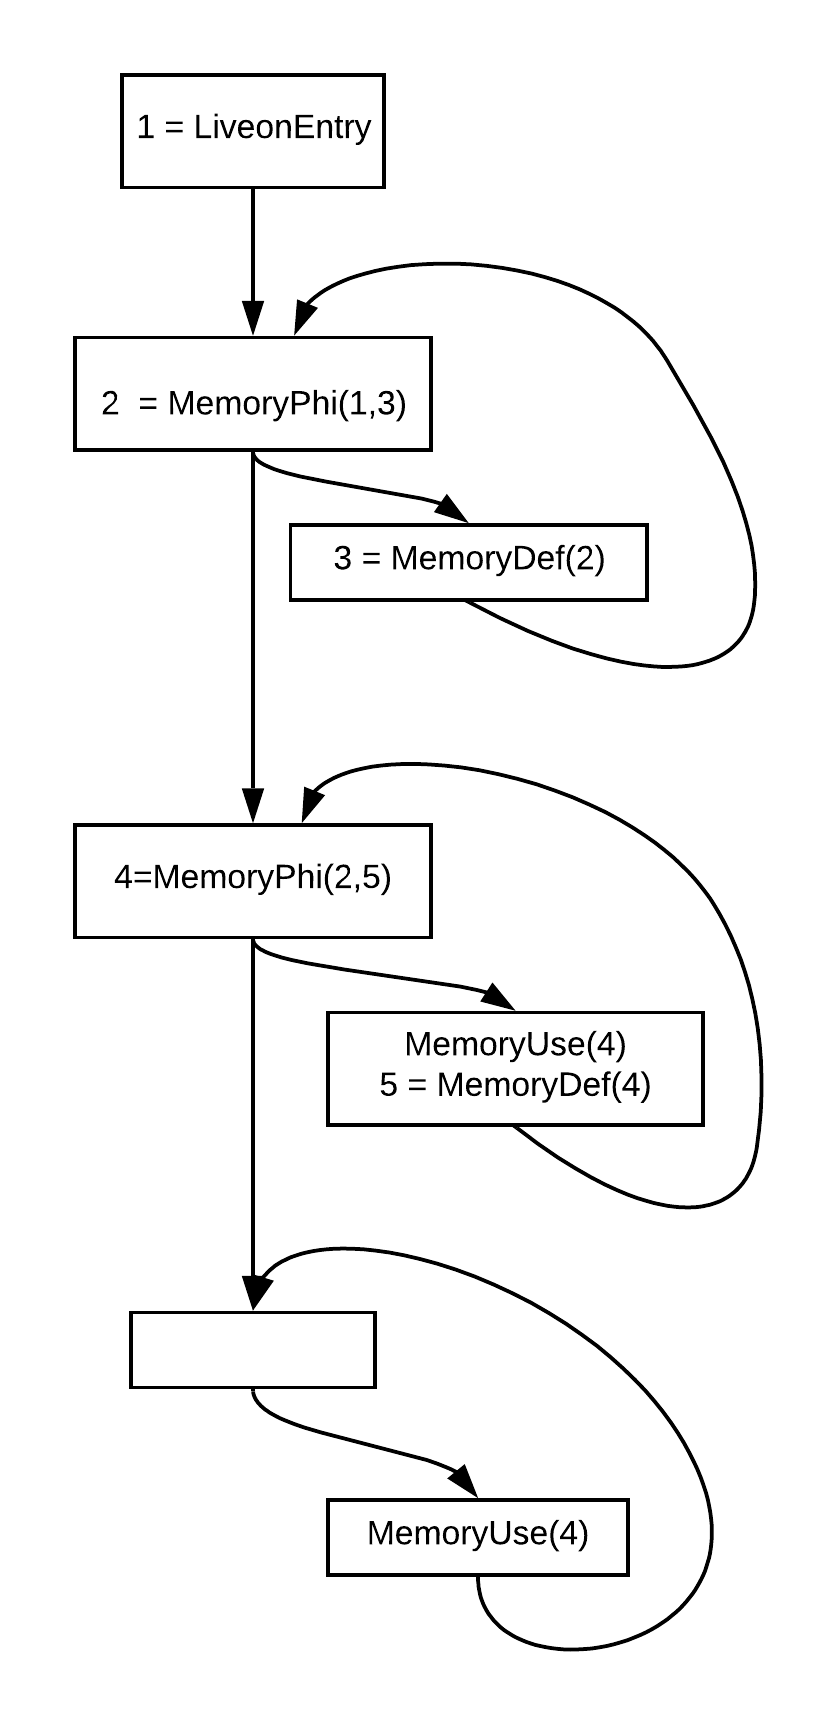
\includegraphics[scale=0.6]{images/memorySSa-impl.png}
\captionof{figure}{Memory SSA of \autoref{memorySSa-impl-code} }
\label{memorySSa-impl}
%         \caption{LLVM Memory SSA Virtual IR}
%         \label{memorySSa-impl}     
%  \begin{figure}
%     \begin{subfigure}{.45\textwidth}
%         \centering
%         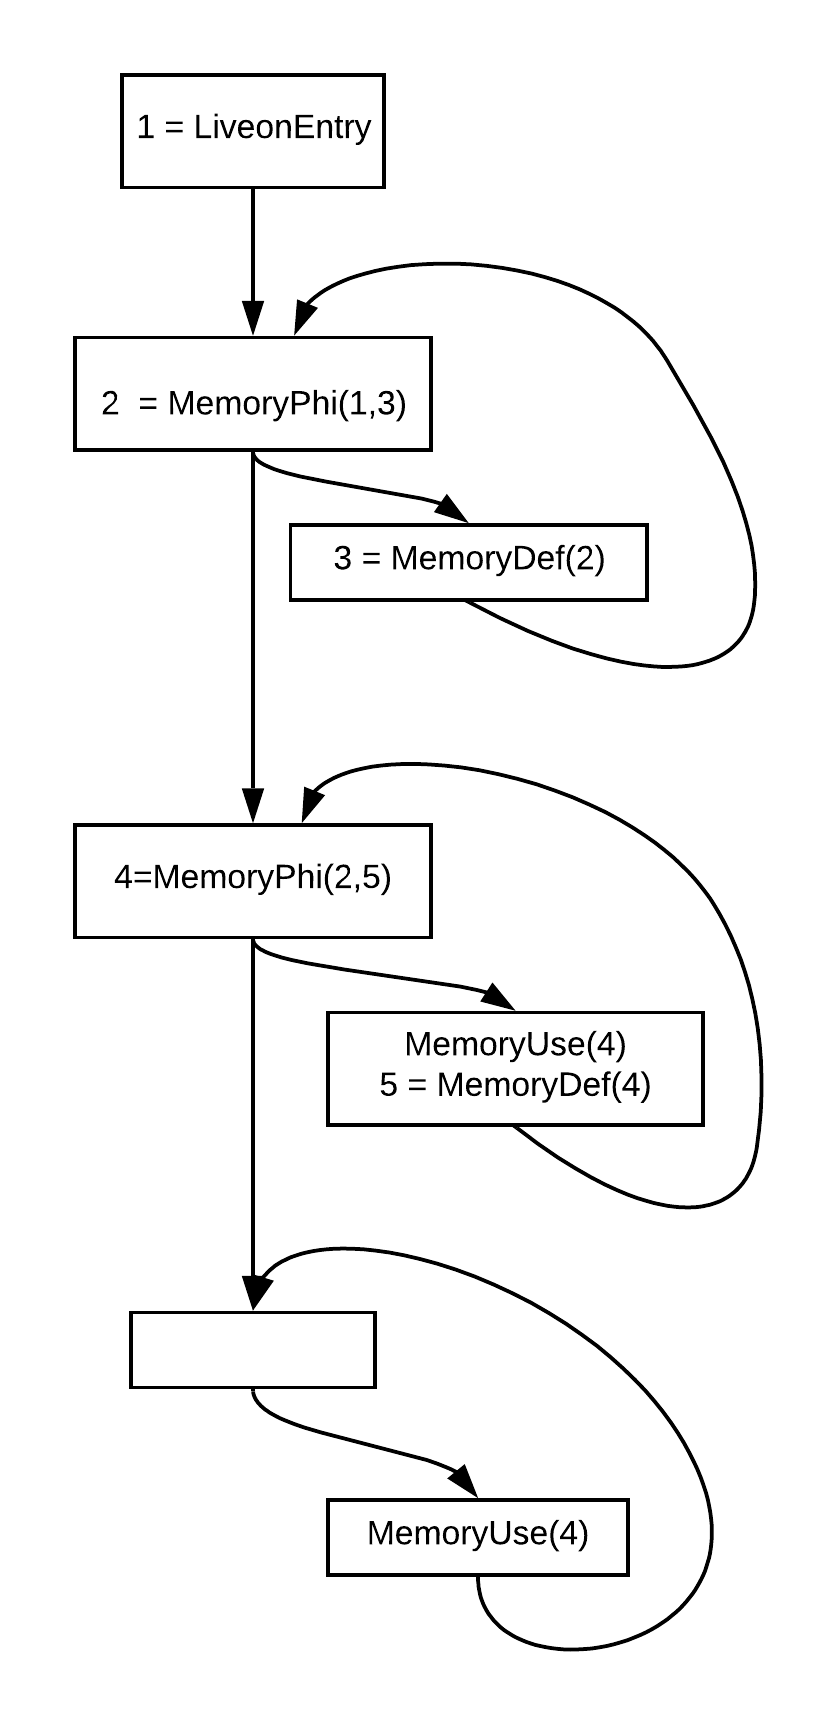
\includegraphics[scale=0.6]{images/memorySSa-impl.png}
%         \caption{LLVM Memory SSA Virtual IR}
%         \label{memorySSa-impl}     
%     \end{subfigure}%
%     \caption{ LLVM MemorySSA Example }
%     \label{LLVMMemorySSA-exmpl}
% %     \vspace{-80pt}
% \end{figure}
\end{minipage}

% \begin{figure}
% %  \hspace*{-10pt}
%     \centering
%     \begin{subfigure}{0.45\textwidth}
%         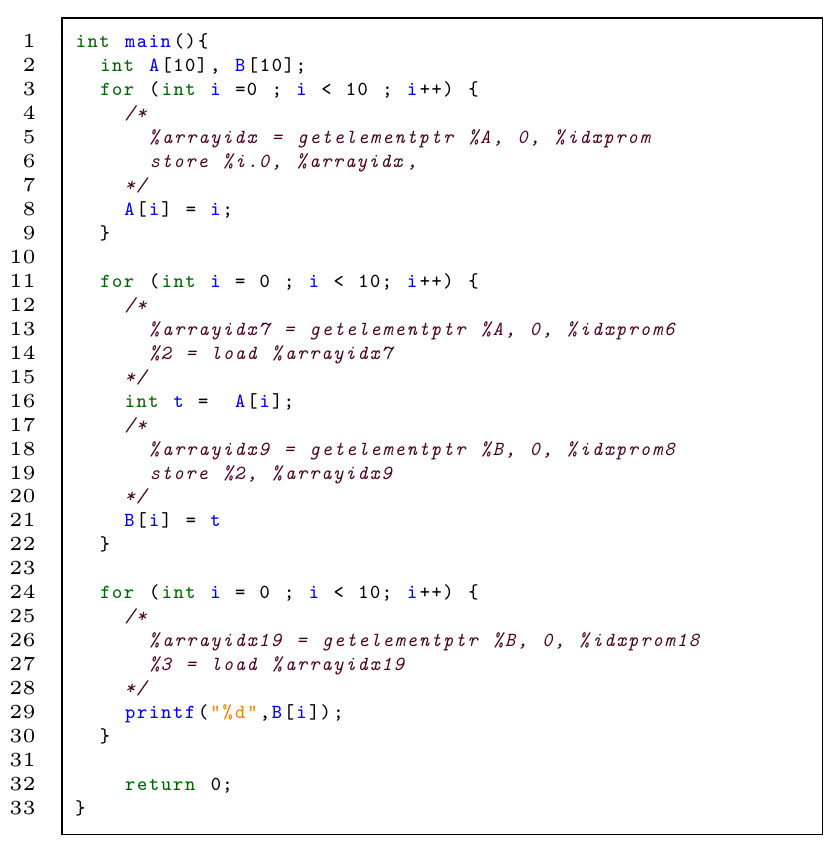
\includegraphics[scale=0.45]{images/memorySSa-impl-code.png}
%         \caption{Code Fragment}
%         \label{memorySSa-impl-code}     
%     \end{subfigure}%    
%     \hspace{40pt}
%     \begin{subfigure}{.45\textwidth}
%         \centering
%         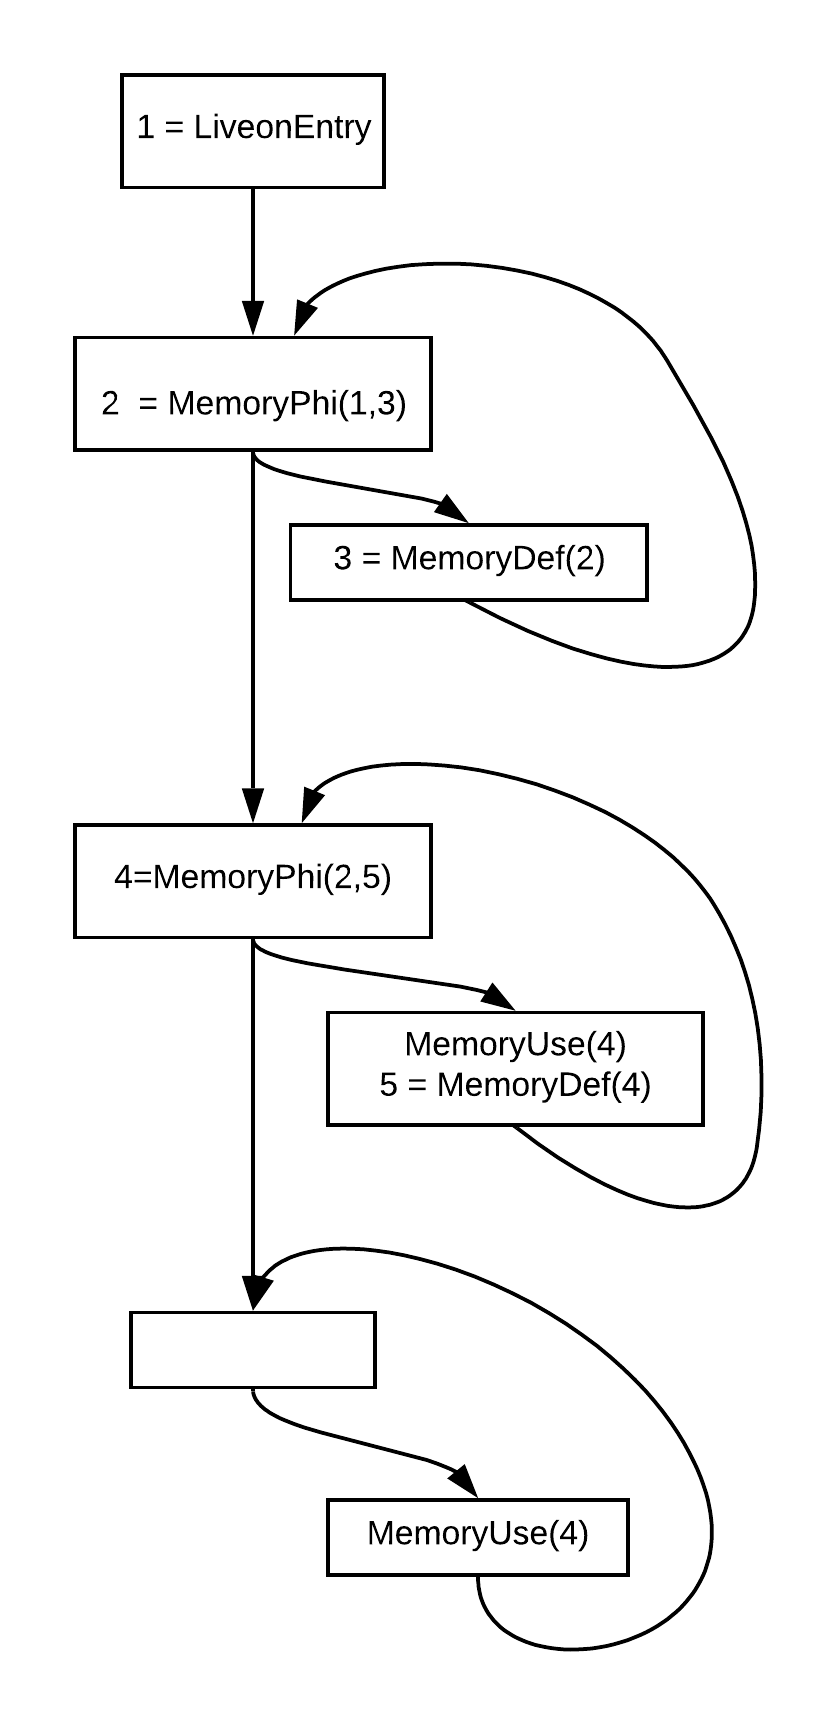
\includegraphics[scale=0.6]{images/memorySSa-impl.png}
%         \caption{LLVM Memory SSA Virtual IR}
%         \label{memorySSa-impl}     
%     \end{subfigure}%
%     \caption{ LLVM MemorySSA Example }
%     \label{LLVMMemorySSA-exmpl}
% %     \vspace{-80pt}
% \end{figure}

Now, we can see the difference between the LLVM memory SSA, 
\autoref{memorySSa-impl} and the array def-use chains  
required for our analysis \autoref{fig:memorySSA-example1}.
We developed a dataflow analysis to 
extract the 
array def-use chains from the LLVM Memory SSA, whenever we can disambiguate the memory variable
that each load/store instruction refers to. 
So, for any store instruction, for example line 22, \autoref{memorySSa-impl-code}, we can analyze the 
LLVM IR, and trace the value that the store instruction refers to, 
which is ``B'' as per the comment in line 19. 
% In this example, line 18, refers to memory variable B, and 
% hence clearly, the $5=MemoryDef(4)$ does not clobber memory variable A. 

We perform an analysis 
on the LLVM IR, which tracks the set of memory variables that each 
LLVM load/store instruction refers to. 
It is a context-sensitive and flow-sensitive 
iterative data flow analysis that associates each MemoryDef/MemoryUse with a set of memory variables. The result of this analysis is an
array SSA form, for each array variable, to tracks its def-use chain, 
similar to the example in \autoref{fig:memorySSA-example1}.
% If the set is a singleton set, then it is a \textit{Must} access, 
% otherwise, it is a \textit{May} access. 
% \begin{minipage}{.45\textwidth}
% \subsection{Validation of data mapping}
% % After the data flow analysis on the memory SSA, we  have the 
% % memory def-use chains. 
% Also, the 
% analysis of \autoref{interpreting-openmp-pragmas} interprets 
% the memory copies introduced by the omp map clauses. Now as explained in 
% section \autoref{s3}, for every pair of Memory def-uses, we 
% verify if the map clause respects that relation. We use the 
% LLVM ''OptimizationRemarkEmitter'' to output the result of our 
% analysis. As we had classified each memory access as must/may, we 
% classify the must violations as Errors, and the may violations as warnings.
% We can prove that the Must violations, found out by our analysis are real bugs in memory mapping 
% clause in the user program.
% \vspace*{-10pt}
\subsubsection{Scalar Evolution Analysis}
LLVM Scalar Evolution is a very powerful technique
that can be used to analyze the change in 
the value of scalar variables over iterations of a loop. 
We can use the SCEV analysis to represent the loop induction variables 
as chain of recurrences. This mathematical representation 
can then be used to analyze the variables used to index into memory 
operations. 
% The SCEV representation in \autoref{memorySSa-impl-code} for variable $i$ on line 16 is `` $\{0,+,1\}<\%for.Line11>$ ''. 
% \begin{itemize}
%  \item The first term of the SCEV is the initial value
%  \item Second term is a mathematical step operation, 
%  in this case it is the increment operator
%  \item Third term is the value which is used to apply the step operation,
%  in this case it is increment by 1,
%  it can also be another SCEV to express chain of recurrences
%  \item SCEV also contains the corresponding enclosing for loops
% \end{itemize}
For our analysis, we need the range of a memory index expression. 
That is the minimum and maximum values, 
of the index expression of any memory address. 
The LLVM SCEV 
analysis can be used to evaluate the maximum value of any variable within 
a loop nest.
to get the maximum number of iterations
of a loop. 
This value can be used to evaluate the maximum value of the SCEV
expression.
We implemented an analysis for array sections, 
that given a load/store, uses the LLVM SCEV analysis, to compute the minimum and maximum values of 
the corresponding index into the memory access. 
% This minimum and maximum can be an expression in terms of program variables. 
% We use this analysis to extract the array sections accessed by any memory load/store. If the SCEV analysis fails to 
% analyze a variable, then we approximate the array section 
% to the maximum size of the array.
% If the memory load/store is from a static array, 
% then the bounds of the array are compile time constants. 
If the analysis fails, then we default to the maximum array size, 
which is either a static array, or can be extracted from the LLVM
memory  \textit{alloc} instructions.
% \vspace{-10pt}
% Otherwise we parse the arguments of the call to memory alloc (malloc), 
% to get the bounds of the corresponding memory variable.
% 
% There are three main cases for the result of SCEV analysis
% \begin{enumerate}
%  \item The upper and lower bounds are compile time constants
%  \item The upper and lower bounds are expressions of program variables
%  \item SCEV is an unknown or cannot be evaluated
% \end{enumerate}
% 
% For our analysis, we approximate the case 2 and 3, with the maximum 
% size of an array. If the memory load/store is from a static array, 
% then the bounds of the array are compile time constants. 
% Otherwise we parse the arguments of the call to memory alloc (malloc), 
% to get the bounds of the corresponding memory variable.
% 
% So, the Array Sections analysis works only if the range of a 
% memory access can be evaluated to compile time integer constants. 
% 
% Finally we use the algorithm from \autoref{dataMapAnalysisAlgo} to warn 
% the user if incorrect array sections are used in the memory map clause.
% The warning can be of the following types
% \begin{itemize}
%  \item Array section accessed on the device environment is larger than the array section mapped onto the device, that is out of bounds access on the device
%  \item Array section mapped out of the device environment to the host, is smaller/subset of what the host environment accesses. 
% \end{itemize}
% __tgt_target_data_begin,3.c:16,3.c:16,0,persistentIn,copyin,A[0:5],persistentOut,copyout,alloc,B[0:10],                                                                                                            
% __tgt_target,3.c:17,3.c:21,0,persistentIn,A[0:10],B[0:10],copyin,persistentOut,copyout,A[0:10],B[0:10],alloc,
